%% 
%% Copyright 2007-2020 Elsevier Ltd
%% 
%% This file is part of the 'Elsarticle Bundle'.
%% ---------------------------------------------
%% 
%% It may be distributed under the conditions of the LaTeX Project Public
%% License, either version 1.2 of this license or (at your option) any
%% later version.  The latest version of this license is in
%%    http://www.latex-project.org/lppl.txt
%% and version 1.2 or later is part of all distributions of LaTeX
%% version 1999/12/01 or later.
%% 
%% The list of all files belonging to the 'Elsarticle Bundle' is
%% given in the file `manifest.txt'.
%% 

%% Template article for Elsevier's document class `elsarticle'
%% with numbered style bibliographic references
%% SP 2008/03/01
%%
%% 
%%
%% $Id: elsarticle-template-num.tex 190 2020-11-23 11:12:32Z rishi $
%%
%%
\documentclass[preprint,12pt]{elsarticle}

%% Use the option review to obtain double line spacing
%% \documentclass[authoryear,preprint,review,12pt]{elsarticle}

%% Use the options 1p,twocolumn; 3p; 3p,twocolumn; 5p; or 5p,twocolumn
%% for a journal layout:
%% \documentclass[final,1p,times]{elsarticle}
%% \documentclass[final,1p,times,twocolumn]{elsarticle}
%% \documentclass[final,3p,times]{elsarticle}
%% \documentclass[final,3p,times,twocolumn]{elsarticle}
%% \documentclass[final,5p,times]{elsarticle}
%% \documentclass[final,5p,times,twocolumn]{elsarticle}

%% For including figures, graphicx.sty has been loaded in
%% elsarticle.cls. If you prefer to use the old commands
%% please give \usepackage{epsfig}

%% The amssymb package provides various useful mathematical symbols
\usepackage{amssymb}
%\usepackage{cite}
\usepackage{amsmath,amsfonts}
\usepackage{algorithmic}
\usepackage{graphicx}
\usepackage{textcomp}
\usepackage{graphics}
\usepackage{caption}

\usepackage{listings}
\usepackage{float}
%%%%%%%%%%%%%%%%%%%
\usepackage{longtable}
\usepackage{booktabs}
\usepackage{lscape} % Para orientación de página horizontal
\usepackage{graphicx} % Para manejar imágenes y gráficos
\usepackage{supertabular}
%% The amsthm package provides extended theorem environments
%% \usepackage{amsthm}

%% The lineno packages adds line numbers. Start line numbering with
%% \begin{linenumbers}, end it with \end{linenumbers}. Or switch it on
%% for the whole article with \linenumbers.
%% \usepackage{lineno}

%%%%%%%%%%%%%%%%%%
\usepackage{graphics}
\usepackage{rotating}
\usepackage{graphicx}
\usepackage{setspace}
\usepackage{epsfig}
\usepackage{listings}
%\usepackage{algorithm}
\usepackage{subcaption}
%%\usepackage{ecrc}
%\usepackage{epstopdf}
%\usepackage[linesnumbered, ruled]{algorithm2e}
%\usepackage[]{algorithm2e}
\usepackage{xurl}
%\usepackage{dcolumn}
%\usepackage{multicolumn}
\usepackage{tabularx}
\usepackage{soul}
\usepackage{booktabs}
%\usepackage{algorithmic}
\usepackage{xcolor}
%\usepackage{algorithm}
\usepackage{listings}
\usepackage{comment}

\journal{International Journal of Transportation Science and Technology}

\begin{document}

\begin{frontmatter}

%% Title, authors and addresses

%% use the tnoteref command within \title for footnotes;
%% use the tnotetext command for theassociated footnote;
%% use the fnref command within \author or \address for footnotes;
%% use the fntext command for theassociated footnote;
%% use the corref command within \author for corresponding author footnotes;
%% use the cortext command for theassociated footnote;
%% use the ead command for the email address,
%% and the form \ead[url] for the home page:
%% \title{Title\tnoteref{label1}}
%% \tnotetext[label1]{}
%% \author{Name\corref{cor1}\fnref{label2}}
%% \ead{email address}
%% \ead[url]{home page}
%% \fntext[label2]{}
%% \cortext[cor1]{}
%% \affiliation{organization={},
%%             addressline={},
%%             city={},
%%             postcode={},
%%             state={},
%%             country={}}
%% \fntext[label3]{}

\title{A Dynamic Geospatial Framework for Four-Level Classification of Urban Intersections Based on Cyclist–Vehicle Accident Severity: A Case Study of the Guadalajara Metropolitan Area}

%% use optional labels to link authors explicitly to addresses:
% \author[label1,label2]{}
% \affiliation[label1]{organization={},
%             addressline={},
%             city={},
%             postcode={},
%             state={},
%             country={}}
%
% \affiliation[label2]{organization={},
%             addressline={},
%             city={},
%             postcode={},
%             state={},
%             country={}}

\author[1]{Ramon A. Briseño}
\ead{rbriseno@up.edu.mx}
%% \ead[url]{home page}
%% \fntext[label2]{}
%% \cortext[cor1]{}
\affiliation[1]{organization={Universidad Panamericana, Facultad de Ingeniería},
            addressline={Álvaro del Portillo 49}, 
            city={Zapopan},
            postcode={45010}, 
            state={Jalisco},
            country={México}}
%% \fntext[label3]{}
\author[2]{Edgar Cossio \corref{cor1}}
\ead{edgar.cossio@iieg.gob.mx}
\cortext[cor1]{corresponding author}
%% \ead[url]{home page}
%% \fntext[label2]{}
%% \cortext[cor1]{}
\affiliation[2]{organization={Instituto de Información Estadística y Geográfica de Jalisco},
            addressline={Calzada de los Pirules 71 Col. Cd. Granja}, 
            city={Zapopan},
            postcode={45010}, 
            state={Jalisco},
            country={México}}
%% \fntext[label3]{}
\author[1]{Carolina Del-Valle-Soto}
\ead{cvalle@up.edu.mx}
%% \ead[url]{home page}
%% \fntext[label2]{}


%% \fntext[label3]{}
\author[4]{Carlos Mex-Perera}
\ead{jmpiee@rit.edu}
%% \ead[url]{home page}
%% \fntext[label2]{}
%% \cortext[cor1]{}
\affiliation[3]{organization={Rochester Institute of Technology},
            addressline={One Lomb Memorial Dr}, 
            city={Rochester}, 
            state={New York},
            country={USA}}
\author[1]{Juan-Carlos L\'opez-Pimentel}
\ead{clopezp@up.edu.mx}

%% \fntext[label3]{}


\begin{comment}
%Previous version
\begin{abstract}
%% Text of abstract
To reduce the mobility carbon footprint in megacities, bicycles for short distances is one of the clean and healthy solution. However, the amount of registered accidents on the road between motorized vehicles and bicycles creates an important concern. Moreover, we present the case of the Guadalajara Metropolitan Area with more than 6 million population, 3 million vehicles, and in the past decade more than 120 km of bicycle lanes looking to provide safety to more than 126,000 bicycle users. To achieve this objective, this work presents three main contributions. 
First, a feature engineering strategy is developed to estimate cyclist flow variables, enriching the original accident dataset with exposure-related information. 
Second, a novel methodology is proposed that transforms the outputs of a machine learning algorithm into a rankable, severity-based process for classifying urban intersections using cyclist–vehicle accident data. 
Third, an online platform is implemented to enable the georeferenced and dynamic identification of high-risk areas by interactively incorporating user-related, temporal, and vehicle-specific variables, 
thereby supporting safety planning through an intuitive and easily interpretable interface.
\end{abstract}
\end{comment}


\begin{abstract}
%% Text of abstract
Reducing the carbon footprint of urban mobility in megacities requires, among other strategies, promoting active transportation modes such as cycling. However, cyclist safety remains a critical challenge, particularly in urban areas where collisions between bicycles and motorized vehicles result in significant fatalities and injuries. In the Guadalajara Metropolitan Area (Mexico), approximately 23 cyclist deaths and 104 injuries are recorded annually, highlighting an urgent road safety concern in a city of over six million inhabitants.

While prior studies have addressed cyclist risk through exposure estimation, georeferenced risk visualization, or binary classification models, these approaches are typically implemented in isolation. This study proposes a unified public decision-support framework that integrates exposure modeling, probabilistic risk estimation, and interactive geospatial visualization to classify urban intersections according to mortality risk in cyclist–vehicle collisions.

By enabling cyclists to identify safer routes and supporting authorities in prioritizing infrastructure interventions, the proposed framework contributes to more efficient allocation of road safety resources and strengthens data-driven decision-making in urban mobility planning.
\end{abstract}


%%Graphical abstract
%\begin{graphicalabstract}
%\includegraphics{grabs}
%\end{graphicalabstract}

%%Research highlights
% \begin{highlights}
% \item This study introduces the RAMCI platform, an innovative real-time predictive system for assessing the severity of cyclist-vehicle accidents in an urban setting using georeferenced machine learning algorithms. The methodology developed in this research represents a significant advancement in traffic safety analysis by integrating diverse data sources, including historical accident records, real-time traffic conditions, and infrastructure characteristics. By leveraging neural networks, logistic regression, and naïve Bayesian models, RAMCI effectively identifies high-risk areas, providing dynamic accident severity predictions through an interactive mapping interface. The platform’s capability to incorporate infrastructure, traffic, and driver-specific variables in a multi-layered prediction approach significantly enhances the accuracy and applicability of accident risk assessment. The findings offer critical insights for urban planners and policymakers, supporting data-driven decision-making to improve cycling infrastructure, implement targeted interventions, and enhance overall road safety.
% \item The impact of this research extends beyond localized accident prevention, contributing to the broader scientific understanding of predictive analytics in transportation safety. Compared to existing global initiatives, RAMCI demonstrates superior efficiency in integrating real-time and spatial data for severity forecasting, establishing a replicable framework for other metropolitan areas. The study's emphasis on key risk factors—such as speed limits, traffic density, road type, and cyclist demographics—aligns with contemporary advancements in intelligent transportation systems, reinforcing the necessity of machine learning applications in urban mobility. By providing an adaptable, evidence-based risk classification model, this research advances state-of-the-art methodologies for cyclist-vehicle accident mitigation, fostering safer and more sustainable urban environments worldwide.
% \end{highlights}

\begin{keyword}
%% keywords here, in the form: keyword \sep keyword

%% PACS codes here, in the form: \PACS code \sep code
%Cyclist-vehicle accident  \sep severity  \sep machine learning \sep online platform \sep methodology.
Cyclist safety \sep Intersection risk modeling \sep Probabilistic classification \sep Decision-support systems \sep Urban mobility planning
%% MSC codes here, in the form: \MSC code \sep code
%% or \MSC[2008] code \sep code (2000 is the default)

\end{keyword}

\end{frontmatter}

%% \linenumbers

%% main text
\section{Introduction}
\label{Changes}

%\hl{El objetivo principal de esta investigación es desarrollar un framework público de apoyo a la toma de decisiones en movilidad ciclista, el cual clasifica las intersecciones del Área Metropolitana de Guadalajara según el riesgo de mortalidad asociado a colisiones entre bicicletas y vehículos motorizados. Este framework permite identificar intersecciones de alto riesgo, facilitando tanto la planificación de rutas más seguras por parte de los ciclistas como la priorización de intervenciones por parte de las autoridades de movilidad y planeación urbana, contribuyendo así a una asignación más eficiente de los recursos destinados a mejorar la seguridad vial.}

%\hl{La problemática es que en el Área Metropolitana de Guadalajara se registran aproximadamente 23 muertes y 104 personas lesionadas en accidentes que involucran bicicletas y vehículos motorizados, lo que evidencia un problema relevante de seguridad vial para los ciclistas en la región.}

The World Health Organization declared in the Global Status Report on Road Safety 2023 that traffic accidents continue to be the leading cause of death worldwide among children and young people aged 5 to 29 \cite{who_global_2023}. Meanwhile, the Pan American Health Organization (PAHO) presented in its report on road safety status in the Americas region, published in June 2019, that the second leading cause of death among young adults aged 15 to 29 is attributed to traffic accidents \cite{pan_american_health_organization_status_2019}. The PAHO also stated that among the 13 middle-income countries where the number of traffic-related deaths increased, Mexico is included \cite{pan_american_health_organization_status_2019}. On the other hand, Mather \cite{mathers_updated_nodate} mentions that the trend in traffic accidents during the period 2016-2060 tends to decrease in high-income countries, however, it increases markedly in middle and low-income countries.

Cyclists, pedestrians, and motorcyclists constitute the most vulnerable sector of the public road \cite{who_global_2023}, having a higher likelihood of dying or suffering serious injury in a traffic accident. In collisions involving different road users, cyclists, pedestrians, and motorcyclists are the most unprotected, receiving impacts directly to their bodies.

To address the issue of cyclists' vulnerability on public roads and tackle other aspects of social impact such as reducing the carbon footprint, promoting physical well-being, and facilitating agile mobility in urban and suburban areas, cities are exploring ways to encourage citizens to use clean mobility, with one of the responses being the creation of bike lanes \cite{mertens_built_2017}.

Thanks to the initiative of active groups, authorities in the Metropolitan Area of Guadalajara, Jalisco, Mexico (AMG) have promoted the creation of bike lanes and a bike-sharing program to encourage cycling mobility \cite{vega_mas_2020}\cite{jalisco_anuncia_nodate}, however, in the AMG, an average of 23 cyclists (from 2009 to 2022) lose their lives annually, and 104 (from 2015 to 2021) are seriously injured in a road accident where at least one motor vehicle is mostly involved \cite{noauthor_datos_nodate}\cite{iieg_mapa_nodate}.

Although cycling infrastructures have proven to be effective in reducing mobility accidents for cyclists, especially when they utilize exclusive lanes that implement safety measures such as separating vehicles and cycling lanes with curbs \cite{mertens_built_2017}, they are not a definitive solution to the issue of cycling mobility accidents. Therefore, government, industry, and academia require greater efforts to ensure that both cycling lanes and roadways in the AMG provide the assurance of being a safe space for mobility accidents for the more than 126,000 citizens who use bicycles as their daily mode of transportation \cite{jalisco_como_vamos_septima_2020}\cite{iieg_cuadernillos_2020}.

Of the three main types of cyclist mobility accident scenarios (single bicycle, bicycle-bicycle, and bicycle-car), encountering a motorized vehicle is the most dangerous for the cyclist's health \cite{Sumit2021}. 
Consulting related work, we found that different authors have addressed cyclist safety from complementary but fragmented perspectives. Several studies emphasize the importance of incorporating cyclist exposure into geospatial analyses, demonstrating that the inclusion of flow-related variables substantially improves predictive performance \cite{ferster_mapping_2021,kielhauser_identifying_2020,xue_integrating_2024}. 
Others define alternative spatial aggregation units, such as grid cells or urban clusters, to identify spatial patterns of crash occurrence and severity \cite{jaber_towards_2023,prencipe_injury_2025}. 
In parallel, research on crash severity prediction has increasingly adopted probabilistic modeling approaches, highlighting the relevance of AUC-based validation and probability-driven risk differentiation rather than relying solely on discrete class labels \cite{ali_advances_2024,schroter_determinants_2023,liu_mixed_2022,scarano_injury_2023,paul_critical_2025}. 
Additionally, hotspot mapping and geospatial visualization techniques are commonly used to communicate risk patterns \cite{ferster_mapping_2021,jaber_towards_2023,prencipe_injury_2025}. 
Although these studies have evidently analyzed cyclist risk through exposure estimation, georeferenced visualization, or classification-based prediction models, these components are typically implemented in isolation. In contrast, we propose a unified public decision-support framework that integrates exposure modeling, probabilistic risk estimation, and interactive geospatial visualization to classify urban intersections according to mortality risk in cyclist–vehicle collisions. By operationalizing these elements within a publicly accessible platform, the proposed approach moves beyond purely analytical contributions and aims to generate actionable tools to safeguard cyclist safety and support infrastructure prioritization.

This work presents a dynamic framework for four-level classification of urban intersections based on cyclist–vehicle accident severity. The proposed framework is composed of a novel methodology for classifying intersections using machine learning algorithms and an online platform that dynamically displays the georeferenced classification, allowing interactive customization through user-related, temporal, and vehicle-specific variables. Through its implemented interactive platform the framework serves as an intuitive decision-support tool that enables governmental authorities to prioritize investments in cycling infrastructure while also assisting citizens in planning safer commuting routes.

The proposed framework focuses on learning calibrated probability outputs from machine learning models trained on infrastructure-related, temporal, user-related, and vehicle-related variables, rather than producing direct binary decisions of accident severity (fatal vs. non-fatal). These predicted probabilities are subsequently used to construct a logically ordered ranking, enabling the transformation of model outputs into four distinct risk levels. Accordingly, model evaluation prioritizes ranking-oriented performance metrics, specifically the Area Under the ROC Curve (AUC) and the Matthews Correlation Coefficient (MCC), instead of accuracy-based measures. Importantly, the dataset is divided into two subsets for training and validation. The validation set is transformed into the same feature space used by the online platform in order to verify the performance of the trained algorithms under real-world operational conditions.


As introductory highlights, the neural network and logistic regression models achieved the best performance among six evaluated machine learning algorithms: Naïve Bayes, Random Forest, Gradient Boosting, Support Vector Machine, neural network, and logistic regression, using a selected subset of variables that includes  \textit{hourly\_range}, \textit{age\_range}, \textit{bicycle\_routes}, \textit{vehicle\_type}, \textit{speed\_limit}, \textit{lanes}, \textit{day}, and \textit{mont}.

This article provides three main contributions: 
\begin{itemize}
    \item A feature engineering strategy is developed to estimate cyclist flow variables, enriching accident records with exposure-related contextual information.
    \item Second, a probabilistic machine learning methodology is introduced to transform predicted probabilities into a four-level, severity-based ranking of intersections, enabling consistent and interpretable risk stratification. 
    \item Third, an open-access online platform is implemented to dynamically visualize high-risk intersections through an interactive map that incorporates temporal, user-related, and vehicle-specific variables.
\end{itemize}


The present work is structured as follows: Section 2 conducts a literature review focused in identifying related studies on methodologies and platforms that classify risk areas or locations for cyclist–vehicle accidents in a georeferenced manner. Section 3, Materials and Methods, describes the feature engineering process used to construct the cyclist–vehicle accident dataset, the methodology employed for intersection severity classification, and the implementation of the georeferenced dynamic platform designed to identify high-risk areas and support safety-oriented decision-making. Section 4 reveals the results and discusses the outstanding findings. Finally, in Section 5, the most important findings of the work are highlighted. 

\begin{comment}
    

\section{Related Works}

Geospatial analyses of cycling mobility have addressed multiple dimensions related to cyclist safety and the development of planning tools. Within this framework, cyclist exposure, particularly bicycle flow volume, has emerged as a critical variable. Studies \cite{ferster_mapping_2021} and \cite{kielhauser_identifying_2020} demonstrate that the inclusion of cyclist exposure substantially improves model accuracy and strengthens performance in real-world applications. Despite its recognized importance, accurately estimating cyclist exposure remains a methodological challenge, particularly in data-scarce urban contexts. 

Cyclist exposure data are commonly obtained from open cloud-based mobility platforms, as in \cite{ferster_mapping_2021}, where bicycle flows are derived from Strava data, or from governmental sources, as in \cite{kielhauser_identifying_2020}, which rely on permanent counting stations. In this study, cyclist flow information is derived from publicly available data from the city’s bike-sharing system MiBici \cite{noauthor_mibici_nodate}. Cyclist exposure datasets differ in coverage and user representation. Crowdsourced platforms such as Strava provide high-resolution activity traces but may reflect only a subset of riders, whereas official bike-sharing data, like MiBici, provide full-system usage but require aggregation and preprocessing. Similar to \cite{xue_integrating_2024}, this work derives likely cyclist trajectories by connecting origin–destination points and estimating the most plausible routes across the urban network.


On the other hand, to represent certain variables in a geospatial framework, previous studies have defined spatial units such as regular grid cells, as in \cite{jaber_towards_2023} or in complete urban areas as in \cite{prencipe_injury_2025}. Like in \cite{xue_integrating_2024} The present proposal adopts intersections as the primary unit of analysis capturing localized risk while aggregating flow and historical crash data within a 200-meter buffer to account for spatial influence.

Among the main geospatial analyses, some illustrate increases and decreases in accidents using counting methods or incident prediction models, as \cite{ferster_mapping_2021} and \cite{kielhauser_identifying_2020}. Some works, such as \cite{schroter_determinants_2023}, \cite{liu_mixed_2022}, and \cite{scarano_injury_2023}, focus on severity prediction with the objective of quantitatively evaluating the impact of predictor variables under different scenarios. For example, \cite{schroter_determinants_2023} analyzes how these variables influence crash severity at signalized intersections, while \cite{liu_mixed_2022} examines how their effects vary between daytime and nighttime conditions.  Others works are distinguished by showing hotspots and identifying high-risk areas based on accident severity, as in \cite{prencipe_injury_2025} and \cite{jaber_towards_2023}. Similarly, this work focuses on classifying risk at intersections based on the severity of past accidents, integrating exposure and historical crash data into a unified geospatial framework. Unlike approaches that remain purely analytical, the proposed framework is fully implemented as an operational system, transforming model outputs into an intuitive and easily interpretable decision-support tool.

Previous studies adopt different methodological strategies to assess cycling safety. \cite{ferster_mapping_2021} divide the network into segments and compares incident counts relative to cyclist exposure across segments. \cite{kielhauser_identifying_2020} analyzes districts over time, predicting expected accident counts and identifying locations that deviate from these predictions. \cite{jaber_towards_2023} aggregates data into grid cells to explore local variations in accident severity, while \cite{prencipe_injury_2025} uses geofenced urban clusters to predict high-severity accident areas. In contrast to previous approaches, and similar to \cite{schroter_determinants_2023},  the present study focuses on intersections, while also integrating feature-engineered cyclist flow and prior accidents within 200-meter buffers to provide a localized assessment of risk.

According to \cite{ali_advances_2024}, many studies adopt probabilistic prediction as a central objective, while validating model performance using metrics such as the Area Under the ROC Curve (AUC), rather than focusing solely on the accuracy of discrete class labels. This probabilistic perspective allows for a more nuanced distinction between different levels of risk in traffic safety analyses. In the present study, where severity is predicted, probability estimates are used instead of class labels to define four classification levels of intersection risk, similar to the approach described by \cite{paul_critical_2025}, which generates vehicular accident risk levels based on predicted probabilities. This probabilistic framework enables a calibrated and interpretable stratification of intersection risk, providing stronger support for decision-making than traditional label-based classification approaches.

Among the reviewed studies \cite{ferster_mapping_2021, jaber_towards_2023, prencipe_injury_2025}, geospatial visualizations, such as hotspot maps or grid-based representations, are explicitly included to illustrate cycling risk across their study areas. 
%However, none of these studies are integrated with an online platform; in contrast, the present work offers a publicly accessible tool that allows residents of the Guadalajara metropolitan area to easily explore and interpret cycling safety data.
\hl{While prior studies have independently addressed cyclist exposure estimation, geospatial risk visualization, and probabilistic prediction through binary classification models, these components have rarely been operationalized within a single, coherent system. The present research bridges this gap by integrating them into a unified decision-support framework that provides a publicly accessible and interactive risk map, explicitly designed to assist both cyclists and mobility authorities in data-driven safety planning.}
\hl{In addition, the tool, implemented with this framework, allows residents of the Guadalajara metropolitan area to easily explore and interpret cycling safety data.}
%\hl{Si bien la generación de exposición ciclista a partir de rutas con origen y destino, la visualización georreferenciada del riesgo mediante mapas y la estimación de probabilidades utilizando algoritmos de clasificación binaria han sido utilizadas previamente en diferentes estudios, la contribución de la presente investigación consiste en integrar estas características en un framework unificado que provee un mapa interactivo público de fácil interpretación, dirigido tanto a la comunidad ciclista como a las autoridades responsables de la toma de decisiones en movilidad ciclista.}
\end{comment}

\section{Related Works}
This section reviews the literature along four complementary dimensions relevant to cyclist safety modeling. First, it examines approaches for estimating cyclist exposure, with particular attention to flow reconstruction from mobility data sources. Second, it discusses the spatial units adopted in geospatial crash analyses, highlighting how different aggregation strategies influence risk representation. Third, it reviews methodological advances in crash severity prediction, emphasizing probabilistic modeling frameworks and evaluation metrics. Finally, it analyzes the extent to which existing studies move beyond analytical modeling toward operational and publicly accessible decision-support systems. This structured review establishes the conceptual and methodological foundations upon which the proposed framework is developed.
\subsection{Cyclist Exposure Modeling}

Geospatial analyses of cycling safety consistently identify cyclist exposure, particularly bicycle flow volume, as a fundamental determinant of crash risk. Incorporating exposure-related variables has been shown to substantially improve predictive accuracy and model robustness in real-world settings \cite{ferster_mapping_2021,kielhauser_identifying_2020}. However, estimating cyclist exposure remains methodologically challenging, especially in urban environments with limited sensing infrastructure.

Existing studies derive exposure data from different sources. Crowdsourced mobility platforms, such as Strava, provide high-resolution activity traces but may represent only a subset of cyclists \cite{ferster_mapping_2021}. In contrast, governmental monitoring systems rely on permanent counting stations that offer structured but spatially limited observations \cite{kielhauser_identifying_2020}. Similar to \cite{xue_integrating_2024}, the present study reconstructs likely cyclist trajectories by connecting origin–destination pairs and estimating plausible routes across the urban network. In our case, cyclist flow is derived from publicly available data from the MiBici bike-sharing system \cite{noauthor_mibici_nodate}, requiring aggregation and preprocessing to obtain exposure indicators at the intersection level.

\subsection{Spatial Units and Geospatial Risk Representation}

The definition of spatial units plays a critical role in geospatial crash analysis. Prior studies have adopted regular grid cells \cite{jaber_towards_2023}, geofenced urban clusters \cite{prencipe_injury_2025}, road segments \cite{ferster_mapping_2021}, or administrative districts \cite{kielhauser_identifying_2020} as primary analytical units. Each approach balances spatial granularity and interpretability differently.

In contrast to grid- or district-based aggregation strategies, and similar to \cite{schroter_determinants_2023}, the present study adopts intersections as the primary spatial unit. Intersections capture localized conflict points between cyclists and motor vehicles while enabling integration of contextual variables. To account for spatial influence beyond the exact node location, cyclist flow and historical crash data are aggregated within a 200-meter buffer surrounding each intersection.

\subsection{Crash Severity Prediction and Probabilistic Modeling}

Beyond descriptive hotspot mapping, recent research increasingly focuses on modeling crash severity and understanding the influence of contextual predictors. Studies such as \cite{schroter_determinants_2023}, \cite{liu_mixed_2022}, and \cite{scarano_injury_2023} examine how roadway, temporal, and demographic variables affect injury severity under different traffic conditions. Other works identify high-risk areas based on severity outcomes using spatial clustering or predictive modeling techniques \cite{jaber_towards_2023,prencipe_injury_2025}.

Methodologically, many contemporary studies adopt probabilistic prediction frameworks and evaluate performance using threshold-independent metrics such as the Area Under the ROC Curve (AUC) \cite{ali_advances_2024}. This probabilistic perspective enables risk differentiation beyond binary class labels. While the literature has embraced continuous risk measures [0,1] from statistical frameworks, as in \cite{paul_critical_2025}, and instance-level probability outputs from machine learning models, as in \cite{zhu_crash_2021,agheli_how_2025}.  The present study uses predicted probabilities rather than discrete outputs to define four ordered levels of intersection mortality risk. This approach supports calibrated and interpretable risk stratification, particularly under class imbalance conditions.

\subsection{From Analytical Models to Operational Decision-Support Systems}

Although prior studies have independently addressed cyclist exposure estimation, geospatial risk visualization, and probabilistic crash prediction, these components are typically developed in isolation. Geospatial visualizations such as hotspot maps or grid-based representations are frequently included to communicate spatial patterns of cycling risk \cite{ferster_mapping_2021,jaber_towards_2023,prencipe_injury_2025}; however, they often remain analytical outputs rather than operational tools.

The present research bridges this gap by integrating exposure modeling, probabilistic severity estimation, and interactive geospatial visualization into a unified decision-support framework. The proposed system is fully operationalized through a publicly accessible platform that enables residents of the Guadalajara Metropolitan Area to dynamically explore intersection-level risk. By transforming model outputs into an intuitive and interpretable interactive map, the framework supports both cyclists and mobility authorities in data-driven safety planning and infrastructure prioritization.

\section{Materials and Methods}
The construction and implementation of the proposed framework consist of three main phases : first phase is, the generation of the database for training machine learning algorithms; the second phase is the methodology to train machine learning algorithms and classify intersection base on cyclist-vehicle accident results; and finally, the implementation of the online dynamic platform to plot the accident severity classification in a georeferenced manner.


\subsection{Database generation}
The database is integrated with information from various sources. Historical accident data involving cyclists and motor vehicles is obtained from the Bicicleta Blanca organization \cite{noauthor_datos_nodate} and the IIEG \cite{iieg_mapa_nodate}. The database also includes information on the amount of cyclist mobility on the roads of the AMG from the open data of the MiBici bike-sharing program \cite{noauthor_mibici_nodate}, and infrastructure information obtained from the platforms Google Maps Street View \cite{noauthor_explora_nodate} and Moovit \cite{noauthor_moovit_nodate}. 

\subsubsection{Collection of information on cyclist mobility accidents}
This stage consists of downloading and storing historical information on cyclist mobility accidents in the AMG. Two Excel spreadsheet files were obtained from the organization Bicicleta Blanca: one with 298 records of fatal accidents from January 2009 to December 31, 2022, and another with 21 records of non-fatal accidents from 2019. Additionally, a CSV file with 39,007 records describing 13,876 fatal and non-fatal traffic accidents from January 2015 to December 2021 was obtained from IIEG. Of the 13,876 traffic accidents recorded in the IIEG, 670 involved a bicycle.


\subsubsection{Unification of sources of historical records of cyclist mobility accidents}
This stage aims to leave all cyclist mobility accident records from the two collected sources (Bicicleta Blanca and IIEG) in a single Excel-type file. The unified file contains 731 records with the following variables and their corresponding classes:

\begin{itemize}
    \item \texttt{Year} in the format \texttt{yyyy}
    \item \texttt{Month-number} in the format \texttt{mm} that can contain the classes \texttt{1, 2, 3, 4, 5, 6, 7, 8, 9, 10, 11,12}.
    \item \texttt{Day} that can contain the classes \texttt{Monday, Thursday, Wednesday Tuesday, Friday, Saturday and Sunday}.
    \item \texttt{Hourly-range} in the format \texttt{00:00 to 00:00}. Ten time ranges were defined: \texttt{0:00 to 05:59, 06:00 to 07:59, 08:00 to 09:59, 10:00 to 11:59, 12:00 to 13:59, 14:00 to 15:59, 16:00 to 17:59, 18:00 to 19:59, 20:00 to 21:59, and 22:00 to 23:59}.
    \item \texttt{Sex} of the bicycle rider (M or F)
    \item \texttt{Age-range} of the bicycle rider with the ranges \texttt{0-19, 20-29, 30-39, 40-49, 50-59, 60+ (60 or more)}
    \item \texttt{Street-type} with the classes Street, Avenue, Peripheral, and Highway.
    \item \texttt{Vehicle-type} with the classes  \texttt{Passenger-vehicle, Private-vehicle, Truck, and Multiple-collision}.
    \item \texttt{Coordx} with the x coordinate that comes from google maps location.
    \item \texttt{Coordy} with the y coordinate that comes from google maps location.
    \item \texttt{Severity} with the classes Injured and Dead.
\end{itemize}

\subsubsection{Compilation of infrastructure variables}
Six different infrastructure variables were collected using Google Maps Street View and the Moovit public transport map. Considering that the infrastructure might have changed from the date of the accident to the present, the Street View with the date closest to the accident was chosen to capture the infrastructure variables that reflect the environment at the time of the accident. Strategy used by previous works like \cite{xue_integrating_2024} to get environment variables. The six added infrastructure variables are as follows:

\begin{itemize}
    \item \texttt{Lanes}: contains the number of lanes of the largest road in the intersection. The generated classes where \texttt{1, 2, 3, 4, 5 and 6+} (six or more lanes).
    \item \texttt{Directions}: contains the number of directions of the largest road in the intersection. The generated classes where \texttt{1, 2} directions.
    \item \texttt{Speed-limit}: expresses the speed limit of the largest road in the intersection. It may contain the classes \texttt{40km/h- (40 km/h or less), 50km/h, 60km/h, and 80km/h.}
    \item \texttt{Bikeway}: contains the classes \texttt{Yes} if any of the streets in the intersection have a bike lane, and \texttt{No} otherwise.
    \item \texttt{Public-transport}: contains the classes \texttt{Yes} if any of the streets in the intersection have public transport routes, and \texttt{No} otherwise.
    \item \texttt{Traffic-light}: contains \texttt{Y}es if there is traffic light signaling at the intersection of the accident, and \texttt{No} otherwise.
\end{itemize}

\subsubsection{Generation of variables cyclist flow, and previous accidents}
Using the open data from the MiBici bike-sharing program, and the Google Maps Directions API, four new variables were generated. Two of them describe the cyclist flow qualitatively and quantitatively, and additionally, two other variables were generated to express the number of cyclist mobility accidents in the zones of each accident record qualitatively and quantitatively.

The cyclist flow variables are: 
\begin{itemize}
    \item \texttt{Bicycle-routes}: indicates the estimated number of cyclists that pass by each accident location per day.

    \item \texttt{Bicycle-routes-cat:} indicates \texttt{Yes} if one or more cyclists pass by the location per day, while \texttt{No} indicates that there is no record of cyclists passing through that location.
\end{itemize}{}

Using the Google Maps Directions API with the bicycle riding option and the origin and destination information of the bike trips from the MiBici program, 15,033 cyclist routes corresponding to March 29, 2023, were generated. The queries to the Directions API have the following format: 

\begin{lstlisting}[breaklines=true]
https://maps.googleapis.com/maps/api/directions/json?origin=20.68722731234884,-103.33410401730704&destination=20.686163379132875,-103.33923240091495&key=REPLACE-API-KEY-HERE&mode=bicycling
\end{lstlisting}


Each of the routes contains the directions with maneuvers, distances, and locations to get from a starting point to a destination point. However, this information is not sufficient to obtain an array of latitude and longitude coordinates uniformly distributed along a route. For this purpose, the overview-polyline field of each route was taken and decoded into a JSON object of ordered coordinates, which represent points to follow along a route with an approximate separation of 100 meters with a ±50 meter accuracy. At this point, having the routes and the route coordinates, it was possible to generate a visualization of the MiBici program routes for the AMG using polylines and a heat map (see figures \ref{fig:routes} and \ref{fig:headmap}). Then, the number of routes that passed within 200 meters or less of each accident record location was counted. For this, an algorithm was used, which, with the help of the Haversine formula equation \ref{eq:Haversine}, calculates the distance in meters between two points on the Earth's surface. For each accident location, the algorithm traverses the coordinates of each polyline corresponding to the 15,030 cyclist routes from March 28, 2023. If at least one coordinate (latitude and longitude) of a polyline is within 200 meters or less of the current accident location, a counter is incremented to quantify the number of cyclist routes near that accident location.


\begin{equation}
\begin{array}{c}
a = \sin^2\left(\frac{\varphi_2 - \varphi_1}{2}\right) + \cos(\varphi_1)  \cdot\cos(\varphi_2)  \cdot\sin^2\left(\frac{\lambda_2 - \lambda_1}{2}\right) \\
c = 2 \cdot \text{atan2}\left(\sqrt{a}, \sqrt{1 - a}\right) \\
\text{distance} = R \cdot c
\end{array}
\label{eq:Haversine}
\end{equation}


Where:
\begin{itemize}
  \item \(\varphi_1\): is the latitude of the first point in radians.
  \item \(\varphi_2\): is the latitude of the second point in radians.
  \item \(\lambda_1\): is the longitude of the first point in radians.
  \item \(\lambda_2\): is the longitude of the second point in radians.
  \item \(R\): is the radius of the Earth in meters (approximately 6,371 km).
  \item \(a\): represents the first term in the Haversine equation, which is the difference in latitude and longitude between two points expressed in terms of sines and cosines.
  \item \(c\): represents the central angle between the two points on the sphere.
\end{itemize}

Figure \ref{fig:bykes} shows the accident quantity visualization map. In this map, for each accident location, a red circle with a radius of 200 meters is drawn, containing at its center a marker with the number of routes that passed within the red area.

\begin{figure*}[h!]
    \centering % centers the figure
    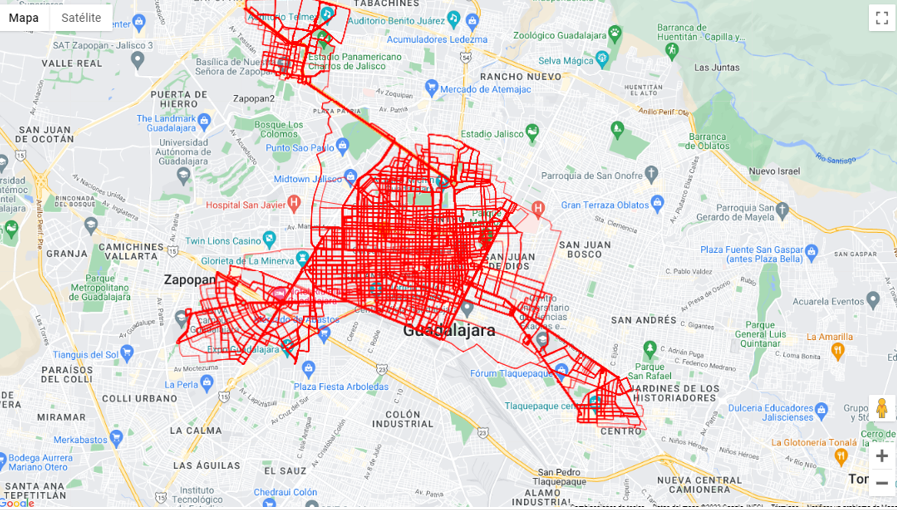
\includegraphics[width=\textwidth]{rutas.PNG} % default size
    \caption{Cyclist routes from the MiBici program of the AMG on March 28, 2023, represented by polylines.} % provides a caption
    \label{fig:routes} % label for referencing the figure
\end{figure*}

\begin{figure*}[h!]
    \centering % centers the figure
    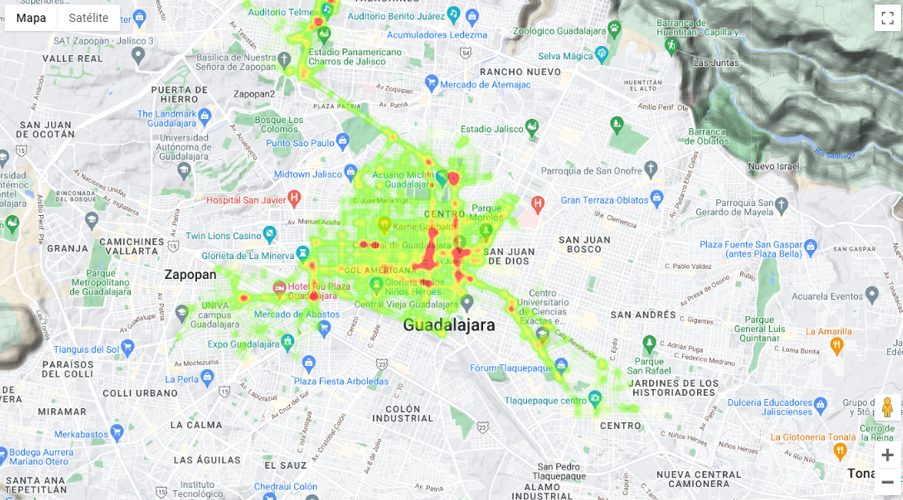
\includegraphics[width=\textwidth]{calor.PNG} % default size
    \caption{Heat map of cyclist mobility in the AMG on March 28, 2023.} % provides a caption
    \label{fig:headmap} % label for referencing the figure
\end{figure*}

\begin{figure*}[h!]
    \centering % centers the figure
    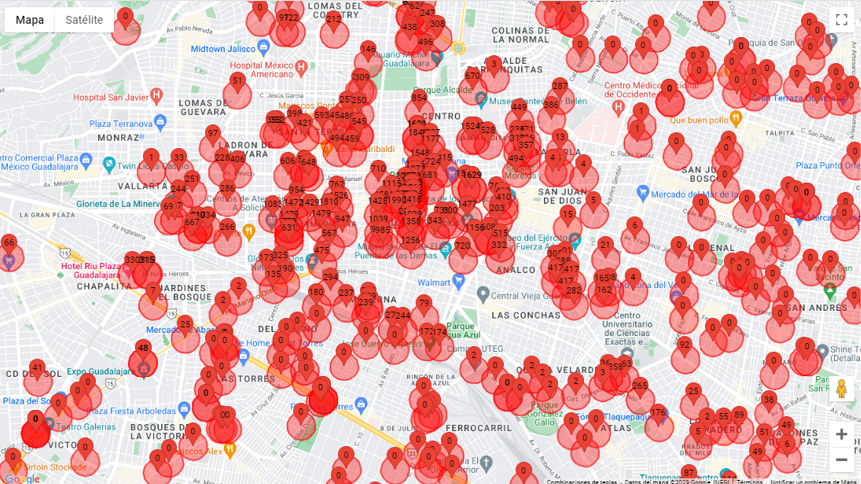
\includegraphics[width=\textwidth]{ciclistas.PNG} % default size
    \caption{Count of cyclist routes on March 28, 2023, that passed through each point where a cyclist mobility accident occurred in the AMG.} % provides a caption
    \label{fig:bykes} % label for referencing the figure
\end{figure*}


Using the same principle as the Haversine formula, for each accident location, the distance to the remaining locations is measured and the number of those within 200 meters or less is quantified. This quantification generates the variables:
\begin{itemize}
    \item \textit{\texttt{Previous-accidents}}: indicates the number of accidents that occurred in the area (within a 200-meter radius) of the accident record location.
    \item \textit{\texttt{Previous-accidents-cat}}: indicates \texttt{Yes} if one or more cyclist mobility accidents occurred at the location, while \texttt{No} indicates that there is no record of other accidents in the area (within a 200-meter radius of the accident location).
  \end{itemize}




\subsubsection{Interpolation}
In the stage of collecting infrastructure variables, the use of Google Maps Open Street View was mentioned for locating the accident on the date closest to the incident, which is beneficial for training the prediction algorithms as it uses the most accurate information possible. However, to predict the severity of a cyclist mobility accident in real time, it is necessary to transfer the knowledge learned from historical data to newly collected, up-to-date information that will feed the proposed platform. This requires re-collecting current data on infrastructure, time, and driver-related conditions. In particular, infrastructure-related variables were gathered again using the current date through Google Maps Street View to ensure consistency with present-day conditions.

\subsubsection{Database description}
This section describes the  distribution of the most important aspects of training dataset variables. 

In the variable \textit{Month-number}, it is noted that there are slightly more accidents during the spring and summer seasons. The variable \textit{Day} shows a trend with non-fatal records; there are more non-fatal accidents on weekdays than on weekends.

9.30\% of the accidents occurred involving women (2.05\% of the "Dead" class and 7.25\% of the "Injured" class), while 84.68\% of the accidents involved men (30.78\% of the "Dead" class and 53.90\% "Injured"). Interesting patterns are observed with the \textit{Age-range} variable; of the 6 age ranges, the range with the most accidents is 20 to 29 years with 24.76\%. Interestingly, 5.06\% are of the "Dead" class while 19.70\% are of the "Injured" class, almost four times more injured than dead.

Considering street infrastructure, more accidents occur on roadways with 1, 2, and 3 lanes, accounting for 21.48\%, 27.77\%, and 30.37\% respectively. However, it is also observed that the number of lanes that provide more safety to a cyclist 6 or more, and 1, as they presented higher proportion of non-fatal accidents. Two-way roads represent 81.94\%, where 29.27\% are fatal accidents and 52.67\% are non-fatal. On one-way streets, deaths make up 4.61\% and injuries 13.41\%. The speed limit has a linear behavior regarding the proportion of deaths in accidents; The higher the speed limit, the greater the proportion of fatal accidents relative to injuries within the same class, except the 50 km/h and 60 km/h classes, which are very similar; however, the 50 km/h class shows a slightly higher number of deaths. In 89.33\% of the accident points, there is no cycling infrastructure. In 58.14\% of accidents, the nearest intersections to the accident point have no traffic lights. In 90.97\% of cases, incidents occurred on a street with the presence of public transport. Lastly, a pattern of fatal accident incidence can be observed in the \textit{Street-type} variable classes; the \textit{Highway} class presents the greatest danger, followed by \textit{Peripheral, Avenue, and Street}.

The most common and dangerous cause of cycling mobility accidents is a collision with a private vehicle with 41.72\%, followed by passenger vehicles with 36.53\%, and heavy trucks with 15.60\%. On the other hand, heavy vehicles are the most fatal followed by passenger vehicles.

In 73.46\% of the records, the \textit{Bicycle-routes-cat} variable shows that the areas of the accidents do not have a detected cyclist flow. Areas with detected cyclist flow are safer than where no flow is recorded.

The time range of the \textit{Hourly-range} variable with the highest number of accidents is from 10:00 to 11:59 AM with 11.35\%, which also is the timeframe with the least fatality (1.37\% for the \textit{Dead} class and 9.99\% for \textit{Injured}). The least frequent and also most fatal time is the early morning from 00:00 to 05:59 AM with a presence of 3.28\% of cases (1.92\% for \textit{Dead} and 1.37\% for \textit{Injured}).

Finally, The target variable severity contains 66.06\% or the records like injured and 33.94\% of the incidents are deaths.



\subsection{Accident severity classification methodology}

The methodological process for training the machine learning algorithms was conducted as follows. The dataset was split into two subsets: 80\% for training and 20\% for validation. A key aspect of this procedure concerns the treatment of missing values. Some records contain null values; however, observations with missing data were not removed from the training set in order to avoid losing potentially valuable information during model learning. In contrast, records with missing values were removed from the validation set. This decision was made to evaluate model performance under the same conditions in which the online platform will operate, where predictions will be generated only from complete user-provided data obtained through platform-based input personalization. 

As an essential component of the methodology, the evaluation strategy is designed to align with the intended use case of the proposed system. This work does not aim to provide a binary prediction of accident severity; instead, it leverages the predict\_proba function of the machine learning models, which outputs a continuous probability value between 0 and 1, where 0 represents the lowest probability of a cyclist being killed and 1 represents the highest probability of a fatal accident.

This probabilistic output enables the construction of a four-level categorical risk index. Predictions between 0.00 and 0.25 are classified as green (low risk), values from 0.26 to 0.50 as yellow (medium-low risk), probabilities between 0.51 and 0.75 as orange (medium-high risk), and predictions from 0.76 to 1.00 as red (high risk).

Given this probabilistic and ranking-based formulation, the evaluation metrics were selected to ensure consistency with the proposed risk-index approach. The Area Under the Receiver Operating Characteristic Curve (AUC) was chosen because it evaluates the model’s ability to correctly rank observations according to their predicted probability, independently of a fixed classification threshold. Since the proposed platform assigns risk categories based on probability intervals rather than a single cutoff point, AUC provides an appropriate measure of how well the model orders cases from lower to higher fatality risk.

Additionally, the Matthews Correlation Coefficient (MCC) was included as a comprehensive metric that considers all elements of the confusion matrix, providing an overall assessment of classification quality. Recall for the fatal outcome was also incorporated due to its importance in identifying high-risk scenarios within the operational context of the platform. Together, these metrics ensure methodological coherence between model evaluation and the intended real-time risk stratification system.

For this purpose, the Orange software [91] was used, which is an open-source platform capable of running machine learning algorithms through the visual programming of components. 6 prediction algorithms were used: Naive Bayes, SVM, Gradient Boosting, Random Forest, Logistic Regression, and Neural Network. The division into training and validation files was done with stratified random sampling, which means that both the training and validation parts maintain their original proportion regarding the \textit{Severity} variable, selecting the records randomly. Although the target class imbalance is not severe, a moderate imbalance exists; thus, higher weights were assigned to the minority class during training to improve its representation in the learning process. 
The selection of predictor features with the best performance was carried out using a backward stepwise methodology and a forward stepwise methodology. 


\subsection{Dynamic web platform implementation}


The Python models of the trained algorithms for severity classification with the best performance and the interpolated database where used to build a back-end four level classification based on the severity prediction probabilities and shows it on a Front-end point-map of the AMG, represented with green, yellow, orange, and red points indicating the intensity of risk at each georeferenced point mapped.

The back-end is composed of an API that predicts accident severity probabilities by responding to requests generated by the front-end, which is dynamically modified according to user input.

The back-end of the system was implemented using the FastAPI framework to handle application logic and API endpoints. The entire back-end is containerized with Docker for consistent deployment across public cloud servers, ensuring scalability and portability. An NGINX server is configured as a reverse proxy to manage incoming requests and enforce TLS encryption, thereby securing API responses and safeguarding communication between clients and the server.

The front-end was developed using the Vue.js framework and deployed on a web hosting platform, providing an interactive interface for users to access and visualize intersection risk data generated by the back-end system.

This setup provides a robust, maintainable, and secure architecture suitable for a cloud-based geospatial risk assessment platform.

The back-end and front-end software repositories are publicly available for consultation, enabling reproducibility and facilitating further development by other researchers \cite{noauthor_general_nodate}, \cite{noauthor_general_nodate-1}.


\section{Results and Discussion}

For the severity prediction process the predictor variables that produced the best performance in the algorithms are: \textit{hourly\_range}, \textit{age\_range}, \textit{bicycle\_routes}, \textit{vehicle\_type}, \textit{speed\_limit}, \textit{lanes}, and \textit{day} for both the Logistic Regression and the Neural Network models. Additionally, the variable \textit{mont} was included exclusively for the Neural Network model. On the other hand, the algorithms that achieved the best combination of AUC and MCC were logistic regression and the neural network.
Table \ref{tab:metrics} shows the percentage of performance for neuronal network and logistic regression.

% Table 10
\begin{table}[H]
\centering
\caption{Performance metrics of prediction algorithms }
\begin{tabular}{|c|c|c|c|c|c|c|}
\hline
\textbf{Algorithm} & \textbf{AUC} & \textbf{CA}& \textbf{F1} & \textbf{Precision} & \textbf{Recall} & \textbf{MCC} \\ \hline Logistic regression
& 88 & 73 & 77 & 87 &73 & 43 \\ \hline
Neural network & 86 & 85 & 87 & 87 & 85 &51 \\ \hline
\end{tabular}
\label{tab:metrics}
\end{table}


The neural network algorithm exhibits slightly better performance metrics than logistic regression; however, logistic regression provides greater interpretability of the data, which is useful for understanding how intersections are classified. For this reason, the web platform employs the predictions produced by the logistic regression model. Figure \ref{fig:nomogram} presents a nomogram that explains variables impact the prediction of the regression model. 

\begin{figure}[h!]
    \centering % centers the figure
    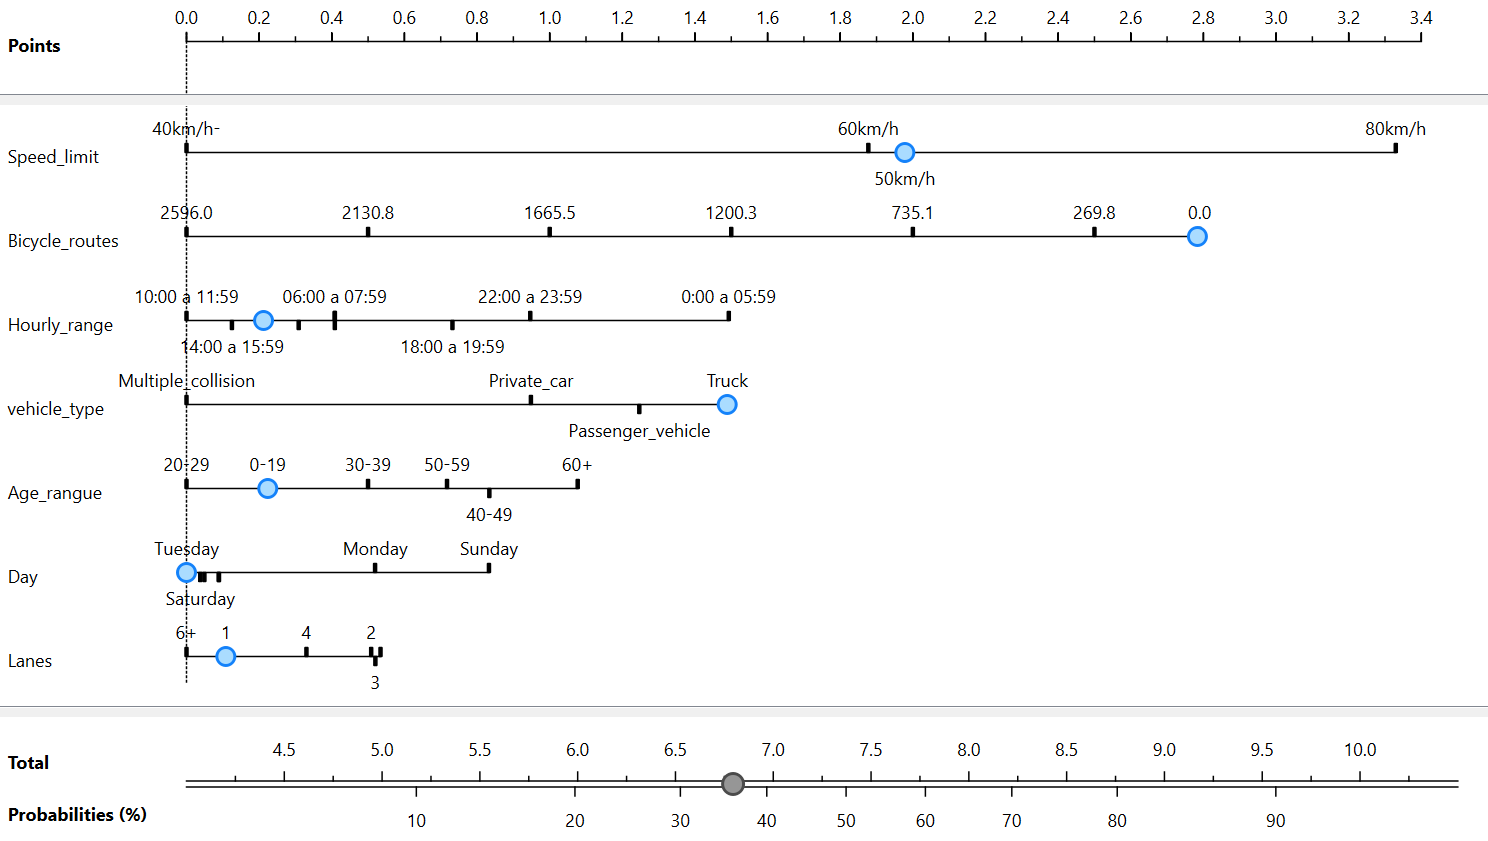
\includegraphics[width=\textwidth]{nomogram.png} % default size
    \caption{Nomogram of the Logistic Regression Algorithm for Predicting the Probability of a Fatal Accident} % provides a caption
    \label{fig:nomogram} % label for referencing the figure
\end{figure}

It can be observed from the nomogram that the variable with the greatest impact on predicting accident fatality is the speed limit, with 80 km/h representing the most dangerous condition and 40 km/h or less being the safest. The presence of cyclist flow provides a meaningful signal to the model: the greater the number of detected bicycle routes, the lower the severity of a potential accident.

Time of day is also a relevant factor. The early morning hours represent the most dangerous period for cyclists, followed by peak traffic hours. In contrast, the time ranges from 10:00 to 12:00 and from 14:00 to 16:00 are identified as the safest periods, as they are associated with lower predicted severity levels.

Regarding vehicle type, freight trucks pose the highest risk, followed by public transportation, private vehicles, and accidents involving multiple vehicles, in that order. In terms of age range, the highest risk corresponds to individuals aged 60 years or older, while the lowest risk is observed in the 20–29 age group. The days associated with the highest risk are Mondays and Sundays. Finally, roadways with a single lane or with six or more lanes are associated with lower risk levels for cyclists.

These findings open the door to the formulation of more complex hypotheses regarding accident behavior and its relationship with severity. For example, the higher risk observed on Sundays and Mondays may be related to accidents occurring during the early hours of the day, potentially reflecting weekend social activities and their spillover into late-night or early-morning travel. An alternative hypothesis points to a potential non-linear relationship between traffic conditions and accident severity, in which extreme traffic conditions, whether characterized by very high or very low volume, are associated with higher predicted fatality risk, while stable and moderate traffic flows correspond to lower severity levels.

Alternatively, Following the graphical interpretation of the classification produced by the online platform, as shown in Figure \ref{fig:mapInfra}, the following findings are observed:
Graphically, a spatial pattern can be observed in the Guadalajara Metropolitan Area. The level of risk classification increases from the city center toward the peripheral zones. The highest risk levels, with nearly all combinations of variables classified as high risk, are observed on the roads that connect to the city’s peripheral beltway.


\begin{figure}[h!]
    \centering % centers the figure
    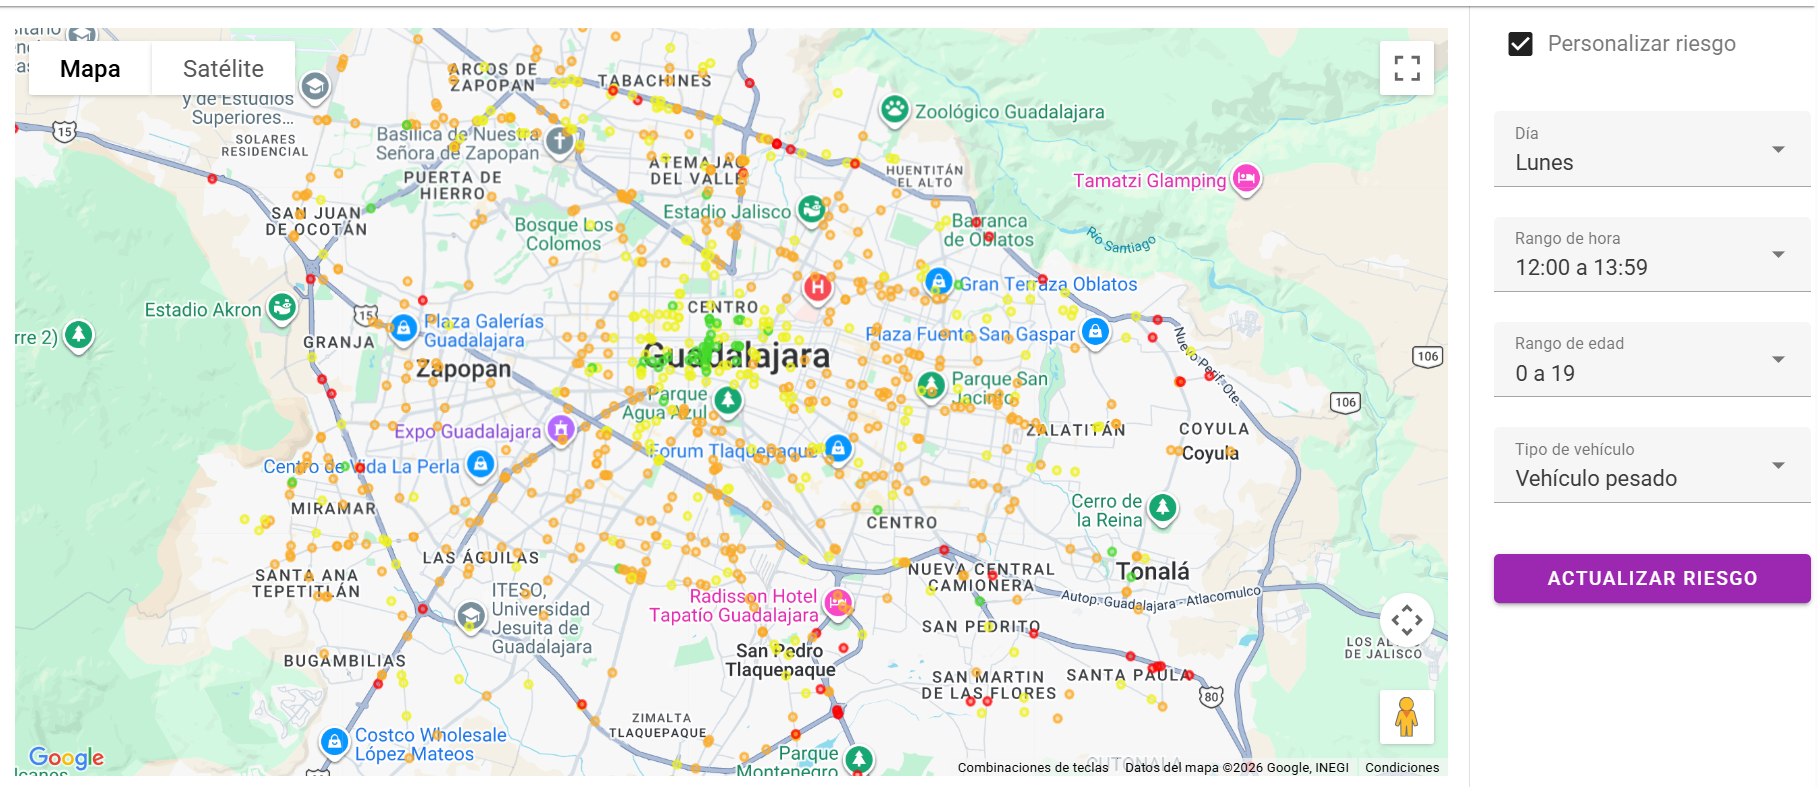
\includegraphics[width=\textwidth]{Dinamico.PNG} % default size
    \caption{Interactive online platform with four level classification} % provides a caption
    \label{fig:mapInfra} % label for referencing the figure
\end{figure}

\subsection{Limitations}

As in the study \cite{wallentin_bicycle-bicycle_2016}, the cyclist flow variable obtained is not complete since it is difficult to identify the exact location of cyclists because they do not regularly use a routing GPS as motor vehicle drivers do. However, the proposed development allowed for accurately identifying how many cyclists pass through any georeferenced point in the city in a day. Beyond the scope of this research, this calculation method could even detect cyclist flow in real-time if there were a direct connection via an API to the MiBici bike-sharing system.


\section{Conclusion}

This study demonstrates that the proposed framework for classifying intersections into four categorical risk levels was successfully developed and validated, providing a practical and interpretable tool for real-time risk assessment. One of the key contribution of this work lies in the feature engineering process, particularly in the construction of variable cyclist flow which enhanced the model's capacity to capture contextual risk patterns. Methodologically, the study emphasized maintaining consistency between model training and real-world deployment. The algorithms were trained using the complete training dataset to preserve as much historical information as possible, while validation was conducted on a modified validation set restricted to complete records, thereby replicating the operational conditions of the web-based platform. Furthermore, model selection was based on the combined evaluation of AUC and MCC. These metrics were chosen because the proposed system does not rely on binary classification outputs; instead, it uses predicted probabilities obtained through the predict\_proba function to rank intersections into four ordered risk levels. In this context, AUC is appropriate because it evaluates the model's ability to correctly rank cases according to predicted risk, independent of a fixed threshold. MCC complements this assessment by providing a balanced measure of overall classification quality, reflecting the model's general predictive support across all confusion matrix components.

Together, these methodological decisions ensure coherence between historical model training, probabilistic risk estimation, and practical implementation within the online platform.

As a result of the model interpretation and the graphical analysis of the platform outputs, it was observed that the variables with the greatest direct impact on classification, according to the logistic regression model selected for deployment, are, in order of importance, speed limit, cyclist flow in the area, time range, vehicle type, age range, day of the week, and the number of lanes on the roadway.

Graphical analysis indicates that roadways with higher speed limits, particularly peripheral roads and highways connecting the city to surrounding areas, are the most dangerous for bicycle travel.

%% The Appendices part is started with the command \appendix;
%% appendix sections are then done as normal sections
%% \appendix

%% \section{}
%% \label{}

%% If you have bibdatabase file and want bibtex to generate the
%% bibitems, please use
%%



\bibliographystyle{elsarticle-num}
\bibliography{bib}

%% else use the following coding to input the bibitems directly in the
%% TeX file.

%\begin{thebibliography}{00}

%% \bibitem{label}
%% Text of bibliographic item

%\bibitem{}

%\end{thebibliography}
\end{document}
\endinput
%%
%% End of file `elsarticle-template-num.tex'.
